\section{Evaluation and Results}
You won't have an evaluation section as developed as Marie. However please describe the results you got : for example ask your parents what they think about this, or ask your siblings to use the prototype and tell us what happened, what did they said. Do not provide names or any personal details, use only their profile like their age and job / hobby / lifestyle/etc if relevant. 
You should create subsections that evaluate different aspects of your project. For example (not all mandatory) : 
\subsection{Design}
... description of what your users said and a final phrase with your analysis and conclusions
\subsection{Interaction}
... description of what your users said and a final phrase with your analysis and conclusions
\subsection{Ergonomics}
... description of what your users said and a final phrase with your analysis and conclusions

You can include tables by zooming and screenshot-ting your screen ( or you can deal with real LateX tables, good luck ) using the same code as for this image.

\begin{figure}[h]
    \centering
    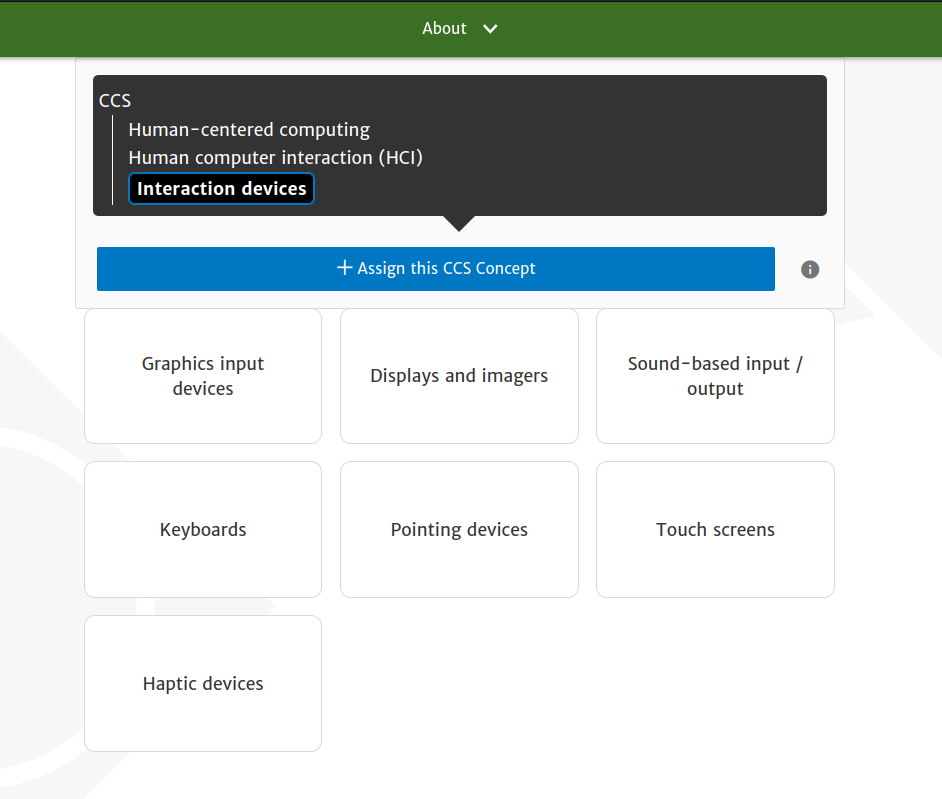
\includegraphics[width=1\columnwidth]{Figures/example.png}
    \caption{Sample image guiding for the choice of concepts on acm website}
    \label{fig:sample}
\end{figure}


